\begin{center}
\Huge
Eksponentiel vækst og fordobling/halvering
\end{center}
\section*{Fordoblings- og halveringskonstanter}
\stepcounter{section}
Perspektivet var før at overveje, hvordan funktionsværdien af eksponentiel vækst udvikler sig, når vi øger $x$ med $1$. Vi kan tilsvarende betragte problemet fra den modsatte side: hvad skal vi øge $x$ med for at fordoble/halvere funktionsværdien. Vi skal altså bestemme en størrelse $T_2$, så 
\begin{align*}
f(x+T_2) = 2f(x)
\end{align*}
for en eksponentialfunktion $f$. Denne idé er præsenteret i Fig. \ref{fig:Fordobling}. 
\begin{figure}[H]
\center
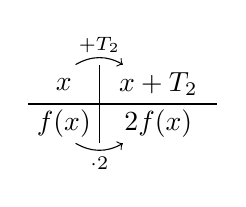
\begin{tikzpicture}
\foreach \i in {0}{
\draw (\i*0.9,0) -- (\i*0.9,1);
}
\draw (-0.9,0.5) -- (1.5,0.5);
\foreach \i in {0}{
\node at (\i*0.9+ 0.75,0.75) {$x+T_2$};
\node at (\i*0.9+0.75,0.25) {$2f(x)$};
}
\node at (-0.45,0.75) {$x$};
\node at (-0.45,0.25) {$f(x)$};
\foreach \i in {0}{
\draw [->] (\i*0.9-0.3,1) to [out=30,in=150] (\i*0.9+0.3,1);
\node at (\i*0.9,1.25) {$\scriptstyle+T_2$};
\draw [->] (\i*0.9-0.3,-0) to [out=-30,in=-150] (\i*0.9+0.3,-0);
\node at (\i*0.9,-0.25) {$\scriptstyle\cdot 2$};
}
\end{tikzpicture}
\caption{Fordoblingskonstant}
\label{fig:Fordobling}

\end{figure}
For eksponentialvækst, hvor fremskrivningsfaktoren $a$ er større end $1$ er det muligt at finde et sådan tal $T_2>0$. Følgende sætning fortæller, hvordan vi skal finde dette tal, og vi kalder tallet for \textit{Fordoblingskonstanten for f}.
\begin{setn}
For en eksponentialfunktion $f$ gælder det, at fordoblingskonstanten $T_2$, der opfylder, at
\begin{align*}
f(x+T_2) = 2f(x)
\end{align*}
er givet ved 
\begin{align*}
T_2 = \frac{\log(2)}{\log(a)} = \frac{\ln(2)}{\ln(a)}
\end{align*}
Tilsvarende er halveringskonstanten $T_{1/2}$, der opfylder, at 
\begin{align*}
f(x+T_{1/2}) = \frac{1}{2}f(x)
\end{align*}
bestemt ved
\begin{align*}
T_{1/2} = \frac{\ln(1/2)}{\ln(a)} = \frac{\log(1/2)}{\log(a)}.
\end{align*}
Desuden gælder der, at $a = \sqrt[T_2]{2}= \sqrt[T_{1/2}]{1/2}$
\end{setn}
\begin{proof}
Vi beviser tilfældet for fordoblingskonstanten. Tilfældet for halveringskonstanten beviset fuldstændig analogt. Lad os derfor for en eksponentialfunktion $f$ givet ved
\begin{align*}
f(x) = b\cdot a^x
\end{align*}
antage, at tallet $T_2$ opfylder, at $f(x+T_2) = 2f(x)$ for alle $x\in \mathbb{R}$. Vi har så, at 
\begin{align*}
f(x+T_2) = 2f(x) \ &\Leftrightarrow \ b\cdot a^{x}a^{T_2}=2b\cdot a^x\\
&\Leftrightarrow\ a^{T_2} = 2\\
&\Leftrightarrow\ \ln(a^{T_2}) = \ln(2)\\
&\Leftrightarrow\ T_2\ln(a) = \ln(2)\\
&\Leftrightarrow\ T_2 = \frac{\ln(2)}{\ln(a)},
\end{align*}
og vi har givet et bevis for fordoblingskonstanten. Siden vi har, at $a^{T_2} = 2$, så må der desuden gælde, at $a=\sqrt[T_2]{2}$, da $a>0$. 
\end{proof}
\section*{Opgave 1}
Bestem fordoblingskonstanten for følgende eksponentialfunktioner
\begin{align*}
	&1) \ 5\cdot 2^x   &&2) \ 7\cdot 0.95^x   \\
	&3) \ 1.03\cdot 1.004^x   &&4) \ 6\cdot 5.09^x   \\
	&5) \ 0.01\cdot 1.75^x   &&6) \ 7.19\cdot 1.179^x   \\		
\end{align*}

\section*{Opgave 2}
\begin{enumerate}[label=\roman*)]
\item Du har 50.000kr på en konto i banken og får 1 procent i årlig rente. Hvor meget står der på din konto efter 12 år?
\item Hvis en bakteriekoloni vokser med 200 procent på et døgn, hvor mange procent vokser den så med på en time?
\item Væksten af en bestemt infektionssygdom er på 2 procent om ugen. Hvad er den månedlige vækst?
\end{enumerate}
\section*{Opgave 3}
Bestem enten fordoblings eller halveringskonstanten for følgende eksponentialfunktioner
\begin{align*}
&1) \ f_1(x) = 0.5\cdot 2^x   &&2) \ f_2(x)=2\cdot 0.5^x  \\
&3) \ f_3(x) = 2000\cdot(0.003)^x  &&4) \ 4e^{27x}  \\
\end{align*}
\section*{Opgave 4}
En bakteriekoloni vokser med $30$ procent i timen. Hvad der fordoblingskonstanten for den eksponentialfunktion, der beskriver antallet af bakterier? Hvad er fordoblingskonstanten, hvis vi ændrer enheden fra timer til dage? Hvad med minutter?

\section*{Opgave 5}
\begin{enumerate}[label=\roman*)]
\item Bevis, at halveringskonstanten $T_{1/2}$ er givet ved 
\begin{align*}
T_{1/2} = \frac{\ln(1/2)}{\ln(a)}
\end{align*}
for en eksponentialfunktion $f(x) = ba^x$. (Hint: Brug beviset for fordoblingskonstanten som skabelon.)
\end{enumerate}